\documentclass[aspectratio=169]{beamer}

\usepackage{pgf}  
\usepackage{tikz}
\usetikzlibrary{arrows}
\usepgflibrary{shapes.arrows} 
\usetikzlibrary{intersections}
\usetikzlibrary{calc}
\usetikzlibrary{fit}
\usetikzlibrary{automata,positioning}
\usepackage{pgfplots,stackengine}
\usepackage{fontspec}
\usepackage{fancyvrb}
\usepackage{wasysym}
\usepackage{unicode-math}
\usepackage{import}
\usepackage{rotating}
\usepackage{gensymb}
\usepackage{chemfig}
\usepackage{rotating}
\usepackage{booktabs}
\usepackage{array}
\usepackage{blkarray}
\usepackage{pifont}
\usepackage{letltxmacro}
\usepackage{wrapfig}
\usepackage{mathtools}
\usepackage{graphbox}
\usepackage{epigraph}
\usepackage{listings}
\usepackage{verbatim}
\usepackage{hologo}
\usepackage{multimedia}
\usepackage[absolute,overlay]{textpos}
\usepackage[euler-digits,euler-hat-accent]{eulervm}
%\logo{\pgfputat{\pgfxy(.45,.5)}{\pgfbox[center]{\includegraphics[width=1.7cm]{Figures/Bioclipse.png}}}}

\usetheme{Copenhagen}
\usecolortheme{beaver}

\definecolor{uured}{RGB}{153,0,0}
\definecolor{darkpastelgreen}{rgb}{0.01, 0.75, 0.24}

\setbeamercolor{block title}{use=structure,fg=white,bg=uured}
\setbeamercolor*{item}{fg=uured}

\newcommand{\unilogo}{
  \setlength{\TPHorizModule}{1pt}
  \setlength{\TPVertModule}{1pt}
  \begin{textblock}{1}(26,-10)
   \includegraphics[height=70pt, align=c]{Figures/uu_shadow.png}
  \end{textblock}
  } 

\pgfmathdeclarefunction{gauss}{2}{%
  \pgfmathparse{1/(#2*sqrt(2*pi))*exp(-((x-#1)^2)/(2*#2^2))}%
}
  
\makeatletter
    \newcases{mycases}{\quad}{%
        \hfil$\m@th\displaystyle{##}$}{$\m@th\displaystyle{##}$\hfil}{\lbrace}{.}
\makeatother

\addtobeamertemplate{frametitle}{}{%
    \unilogo
}

\LetLtxMacro{\oldBlock}{\block}
\LetLtxMacro{\endoldBlock}{\endblock}
\renewcommand{\block}{\begin{center}\begin{minipage}{0.8\textwidth}\oldBlock}
\renewcommand{\endblock}{\endoldBlock\end{minipage}\end{center}}
\setlength{\fboxsep}{0pt}

\begin{document}
\graphicspath{{Figures/}}
\setsansfont[ItalicFont = Optima Italic,
             BoldFont = Optima Bold,
             Ligatures=TeX ]
            {Optima Regular}
\setmainfont[ItalicFont = Optima Italic,
             BoldFont = Optima Bold,
             Ligatures=TeX]
            {Optima Regular}
%\newfontfamily\comment[]{Chalkboard}
\newfontfamily\zA[Ligatures={Common, Rare}, Variant=1] {Zapfino}
\newfontfamily\zB[Ligatures={Common, Rare}, Variant=2] {Zapfino}
\newfontfamily\zC[Ligatures={Common, Rare}, Variant=3] {Zapfino}
\newfontfamily\zD[Ligatures={Common, Rare}, Variant=4] {Zapfino}
\newfontfamily\zE[Ligatures={Common, Rare}, Variant=5] {Zapfino}
\newfontfamily\zF[Ligatures={Common, Rare}, Variant=6] {Zapfino}
\newfontfamily\zG[Ligatures={Common, Rare}, Variant=7] {Zapfino}
\renewcommand\UrlFont{\color{blue}}
\renewcommand\thefootnote{\textcolor{uured}{\arabic{footnote}}}
\setbeamercolor{alerted text}{fg=uured}
\lstset{basicstyle=\ttfamily\scriptsize, frame=single }
\newcommand{\TikZ}{{\lmr Ti\textit{k}Z}}


\title{Ligand-based modeling}   
\author{Jonathan Alvarsson} 
\titlegraphic{\includegraphics[height=18pt]{Figures/pharmbio-logo-new.png}}
\date{\today} 

\setbeamertemplate{background}{%
    \parbox[c][\paperheight]{\paperwidth}{%
        \vfill
        \hfill
        \includegraphics[height=0.65\textheight]{Figures/sigill.png}
    }   
}
\begin{frame}[plain]
\unilogo \vspace{1cm} \titlepage
\begin{tikzpicture}[remember picture,overlay]
\tikz[remember picture, overlay] \fill[uured] (current page.north west) rectangle ++(\paperwidth,-0.5cm);
\end{tikzpicture}%
\end{frame}

\setbeamertemplate{background}{}
\renewcommand{\unilogo}{
  \setlength{\TPHorizModule}{1pt}
  \setlength{\TPVertModule}{1pt}
  \begin{textblock}{1}(0,0)
   \includegraphics[height=27pt, align=c]{Figures/uu.png}\includegraphics[height=10pt, align=c]{Figures/pharmbio-logo-new.png}
  \end{textblock}
  }

    %\begin{frame}
    %\frametitle{Outline}
    %\begin{minipage}{0.25\textwidth}
    %\mbox{}
    %\end{minipage}
    %\begin{minipage}{0.6\textwidth}
    %\tableofcontents
    %\end{minipage}
    %\end{frame}
    
    \begin{frame}
        \frametitle{Ligand-based modelling}
        \framesubtitle{No target and no structure}

        \begin{block}{Ligand-based modelling}
            \begin{itemize}
                \item In ligand-based modelling we are working without a known target
                \item A series of ligands have a certain effect
            \end{itemize}
        \end{block}
    \end{frame}
    
    \begin{frame}
        \frametitle{Ligand-based modelling}
        \framesubtitle{Similarity principle}

        \begin{block}{Similarity principle}
            \begin{itemize}
                \item Similar substances should behave in a similar fashion
                \item What can we learn by just studying the ligands?
            \end{itemize}
        \end{block}
    \end{frame}

\section{QSAR}

    \begin{frame}
        \frametitle{QSAR}
        \framesubtitle{Quantitative structure–activity relationship}

        \begin{block}{Quantitative structure–activity relationship}
            In QSAR we mathematically describe molecular structure and by machine learning predict molecular properties
            \uncover<2>{
            \begin{itemize}
                \item \alert{QSAR} -- Quantitative Structure-Activity Relationship
                \item \alert{QSPR} -- Quantitative Structure-Property Relationship
            \end{itemize}
            }
        \end{block}
    \end{frame}
    
    \begin{frame}
        \frametitle{QSAR}
        \framesubtitle{Quantitative structure–activity relationship}

        \begin{block}{Quantitative structure–activity relationship}
            QSAR can be used for predicting almost any molecular properties:
            \begin{itemize}
                \item Biological activity
                \item Risk management, toxicology
                \item \ldots
            \end{itemize}
        \end{block}

    \end{frame}


    \begin{frame}
        \frametitle{QSAR}
        \framesubtitle{Quantitative structure–activity relationship}
        \centering

        \begin{tikzpicture}
                \node (structures) [text width=2.4cm, rectangle, text centered]
                                  {Molecular structures};
                \node (activity) [text width=3cm, rectangle, 
                                text centered, right of=structures, node distance=3.5cm]
                                {Activity or Property};
                \only<1>{\draw [->] (structures) to (activity);}
                \uncover<2->{\draw [dashed,->] (structures) to (activity);}
            \uncover<2->{
                \node (descriptors) [text width=2.4cm,rectangle, node distance=1.5cm,
                                     text centered, below of=structures]
                                    {Molecular descriptors};
                \draw [->] (structures) to (descriptors);
            }
            \uncover<3->{
                \node (model) [text width=3cm,rectangle, node distance=1.5cm,
                                     text centered, below of=activity]
                                    {Mathematical model};
                \draw [->] (descriptors) to (model);
            }
            \uncover<4->{
                \draw [->] (model) to (activity);
            }
            \uncover<5->{
                \footnotesize
                \node (combine) [text width=3.5cm,rectangle, node distance=2.2cm,
                                     text centered, below left of=descriptors]
                                {\color{darkpastelgreen}Good to combine many different descriptors};
                \draw [->, darkpastelgreen] (combine) to (descriptors);
                \node (validation) [text width=5.6cm,rectangle, node distance=2.2cm,
                                     text centered, below right of=model]
                                {\color{darkpastelgreen}Machine learning};
                \draw [->, darkpastelgreen] (validation) to (model);
                \node (more) [text width=4cm,rectangle, node distance=2cm,
                                     text centered, above left of=structures]
                                {\color{darkpastelgreen}More structures often lead to better models};
                \draw [->, darkpastelgreen] (more) to (structures);
            }
        \end{tikzpicture}
\end{frame}

\section{Molecular Descriptors}
    \begin{frame}
        \frametitle{Molecular Descriptors}
                \begin{block}{Molecular descriptors} 
A molecular \alert{descriptor} is a \alert{mathematical representation} of a
molecule, often resulting from the \alert{transformation} of the \alert{symbolic
representation} of a molecule into \alert{numbers}
        \end{block}
    \uncover<2->{
    \begin{block}{Simple examples}
    \quad
    \begin{minipage}[c]{0.3\linewidth}
        \includegraphics[width=1\textwidth]{figures/paracetamol.png}
    \end{minipage}
    \qquad
    \begin{minipage}[c]{0.4\linewidth}
    \small
    \begin{tabular}{lr}
    \toprule
    Descriptor & Value \\
    \midrule
    Molecular weight          & 151.06 \\
    Number of carbon atoms    & 8      \\
    \bottomrule
    \end{tabular}
    \end{minipage}
    \end{block}}

    \end{frame}

\subsection{Classifications}
       \begin{frame}
        \frametitle{Molecular Descriptors}
        \framesubtitle{Classifications}
        \begin{minipage}[c]{0.6\textwidth}
        \oldBlock{By ``dimensionality''}
        \begin{itemize}
            \item 0D -- molecular weight, number of atoms
            \item 1D -- fragment counts, fingerprints
            \item 2D -- topological descriptors
            \item 3D -- geometrical descriptors
        \end{itemize}
        \endoldBlock
        \end{minipage}
        \hfill
        \begin{minipage}[c]{0.35\textwidth}
        \oldBlock{By data type}
        \begin{itemize}
            \item Boolean
            \item Integer
            \item Real number
            \item Vector
        \end{itemize} 
        \endoldBlock
        \end{minipage}

    \end{frame}

    \begin{frame}
        \frametitle{Molecular Descriptors}
        \framesubtitle{Classifications of descriptors}
        \small
        \begin{block}{Other classification schemas include, \textit{e.g.}, the following classes:}
            \begin{itemize}
                \item Constitutional -- does not take molecular geometry into account
                \item Topological -- based on molecular graphs
                \item Geometrical -- based on 3D structure
                \item Electronic -- based on electronic structure
                \item Physiochemical -- based on lab measurable properties
            \end{itemize}
        \end{block}
        \centering
        \uncover<2->{\color{darkpastelgreen}Classes overlap and descriptors belong to more than one class}
    \end{frame}

\subsection{Examples}

    \begin{frame}
        \frametitle{Molecular descriptors}
        \framesubtitle{Examples}
                \hfill
        \begin{minipage}[c]{0.7\textwidth}
        \oldBlock{Log P}
        \alert{Log P} is a real number physiochemical descriptor. Log P is the
        logarithm of the \alert{partition coefficient}; the the \alert{ratio of
        concentrations} of the studied substance between \alert{water} and
        \alert{octanol}. This affects how easily a drug can reach its intended
        target in the body.
        \endoldBlock
        \end{minipage}
        \hfill
        \begin{minipage}[c]{0.2\textwidth}
        \fbox{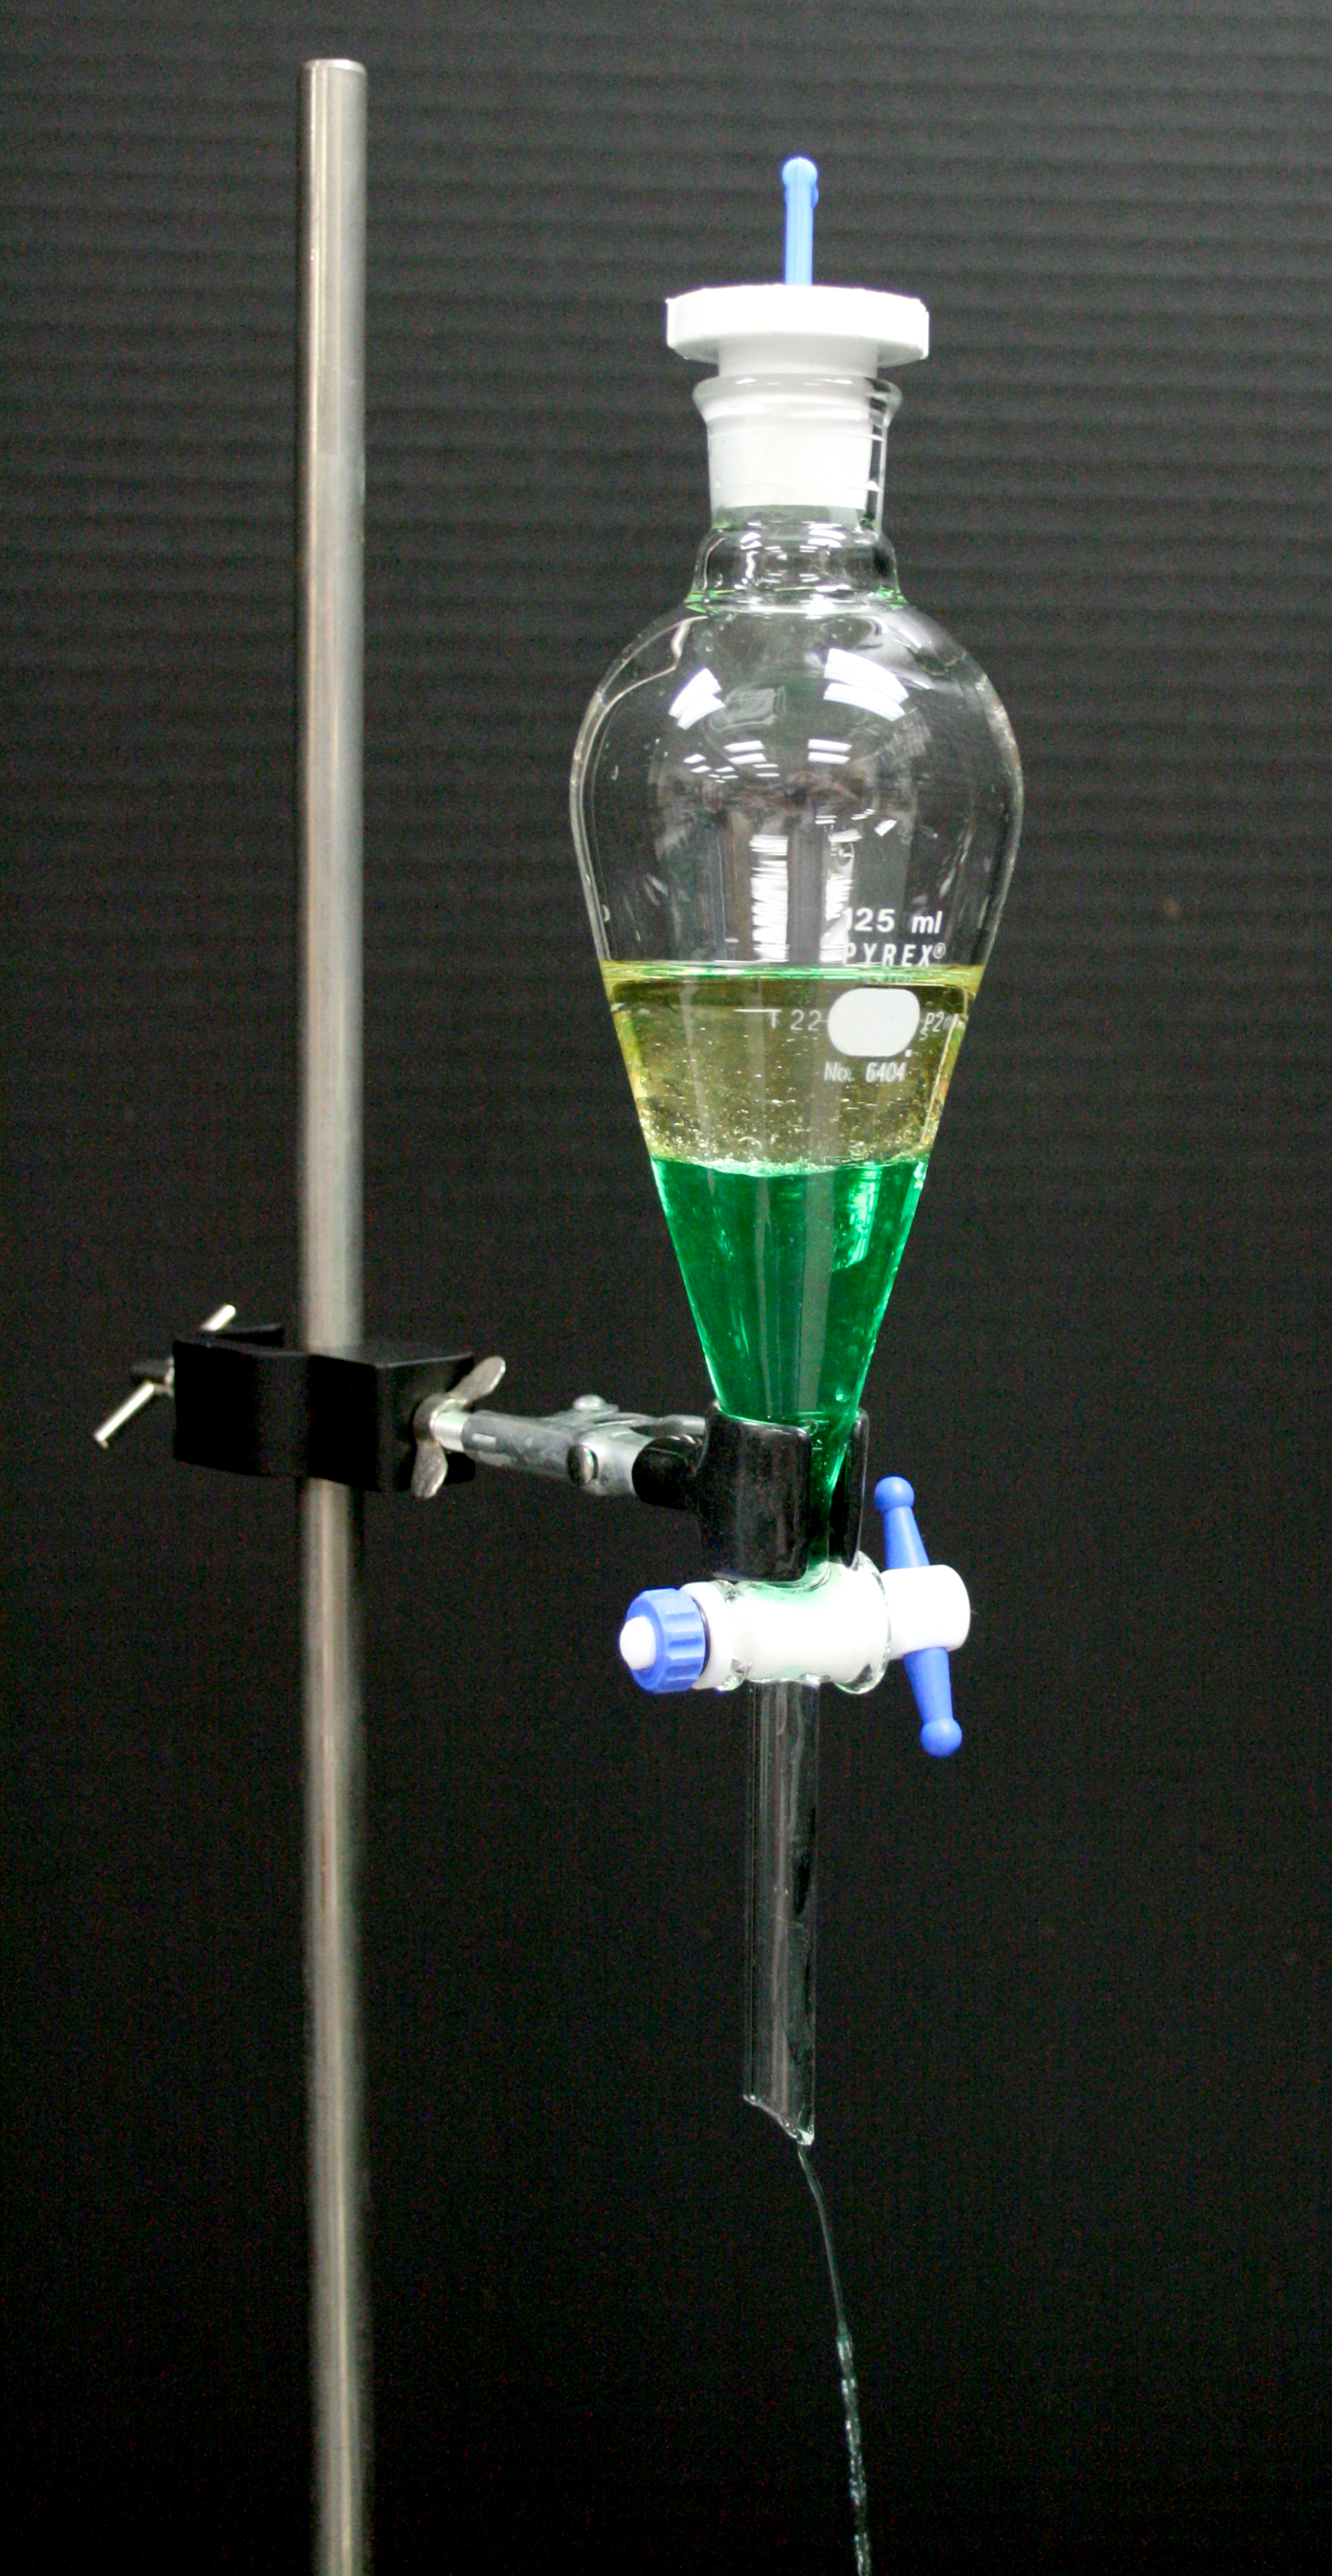
\includegraphics[width=1\textwidth]{Figures/funnel.png}}~\rotatebox{90}{\tiny Photo: \texttt{PRHaney}}
        \end{minipage}
        \hfill
    \end{frame}

    \newcommand\tm[2][]{\tikz[overlay,remember picture,baseline=(#1.base),inner sep=0pt]\node(#1){$#2$};}

    \begin{frame}
        \frametitle{Molecular descriptors}
        \framesubtitle{Examples}
        \begin{block}{Wiener index}
        The \alert{Wiener index} $W$ is defined as: the \alert{sum of the lengths} of the
        \alert{shortest paths between} all \alert{pairs of vertices} in the
        chemical graph of the molecule \alert{excluding hydrogens}. It can be
        calculated by \alert{summing the upper right triangle} of the
        \alert{distance matrix} $D$ for the compound:
        \small
        \begin{equation*}
            D\left( \raisebox{-2ex}{\chemfig{ C_a-C_b-[:50,,,1]O_cH }}\right)  = \begin{blockarray}{cccc}
        & \chemfig{C_a} & \chemfig{C_b} &  \chemfig{O_c} \\
            \begin{block}{c(ccc)}
        \chemfig{C_a} &  0 & \tm[a]{1} & \tm[b]{2} \\
        \chemfig{C_b} &  1 & 0 & \tm[c]{1}         \\
        \chemfig{O_c} &  2 & 1 & 0 \\
        \end{block}
        \end{blockarray},\qquad
        W = 1 + 2 + 1 = 4
        \end{equation*}
        \begin{tikzpicture}[overlay, remember picture]
        \node(x)[fit=(a) (b),inner sep=2pt]{};
        \node(y)[fit=(b) (c),inner sep=2pt]{};
        \fill[rounded corners,opacity=.3,fill=uured](x.north west)--(x.south west)--(y.south west)--(y.south east)--(x.north east)--cycle;
        \end{tikzpicture}
        \vspace{-1\baselineskip}
            \end{block}
    \end{frame}

    \begin{frame}
        \frametitle{Molecular descriptors}
        \framesubtitle{Examples}
        \begin{block}{Signature descriptor}
        The \alert{signature descriptor} is a \alert{topological} descriptor using atom type
        information and represented as a list of strings. It is constructed by describing
        the \alert{environment around each atom} in a molecule by describing each atoms
        \alert{neighbouring atoms} out to a specific distance (refered to as
        height). Hydrogens are often skipped.
        \end{block}
    \end{frame}

    \begin{frame}
        \frametitle{Molecular descriptors}
        \framesubtitle{Examples}

        \oldBlock{Atom Signature descriptor for \chemfig{N_a}}
            \hfill
            \begin{minipage}[c]{0.2\textwidth}
            \chemfig{
                    O_fH% 6
           -[:90,,1]C_d% 1
              -[:36]C_e% 2
            =^[:108]N_a% 3
             -[:180]C_b% 4
    =^[:252.1,0.995]N_c% 5
                       (
         -[:323.7,0.7]% -> 1
                       )
} 
            \end{minipage}
            \hfill
            \begin{minipage}{0.7\textwidth}
\begin{tikzpicture}[level distance=1cm,
  level 1/.style={sibling distance=2cm},
  level 2/.style={sibling distance=1cm},
  level 3/.style={sibling distance=1cm}]
  \node(a) {\chemfig{N_a}}
    child {node {\chemfig{C_b}}
      child {node {\chemfig{N_c}}
        child {node {\chemfig{C_d}}}
        }
    }
    child {node {\chemfig{C_e}}
        child {node {\chemfig{C_d}}
            child {node {\chemfig{N_c}}}
            child {node {\chemfig{O_f}}}
        }
    };
    \node(h1)[right of=a, node distance=4cm]{h=0 [N]};
    \node(h2)[below=of h1.west, anchor=west, node distance=1cm]{h=1 [N]([C],[C])};
    \node(h3)[below=of h2.west, anchor=west, node distance=1cm]{h=2 [N]([C]([N]),[C]([C]))};
\end{tikzpicture}
            \end{minipage}
            \hfill
        \endoldBlock
    \end{frame}



    \begin{frame}
        \frametitle{Molecular descriptors}
        \framesubtitle{Examples}
        \oldBlock{Atom signature descriptors for ethanol}
            \hfill
            \begin{minipage}[c]{0.2\textwidth}
            \chemfig{ C_a-C_b-[:50,,,1]O_cH } 
            \end{minipage}
            \hfill
            \begin{minipage}{0.7\textwidth}
            \begin{tabular}{cccc}
            \toprule
            Height & \chemfig{C_a} & \chemfig{C_b} & \chemfig{O_c} \\
            \midrule
            0      & [C] & [C] & [O] \\ 
            1      & [C]([C]) & [C]([C][O]) & [O]([C]) \\
            2      & [C]([C]([O])) & [C]([C][O]) & [O]([C]([C])) \\
            \bottomrule
            \end{tabular}
            \end{minipage}
            \hfill
            \vspace{1\baselineskip}

            Notice that ethanol is so small that signature heights beyond
            height 2 does not add any more information.
        \endoldBlock
    \end{frame}






\subsection{Molecular Fingerprints}

    \begin{frame}
        \frametitle{Molecular Fingerprints}
    \end{frame}

\section{The QSAR Dataset}
    \frame{
        \frametitle{title}
        \framesubtitle{subtitle}
    }

\end{document}
